\documentclass[a4paper,11pt]{article}

\usepackage{amsmath,amsfonts}
\usepackage{biblatex}
\addbibresource{ref.bib}
\usepackage{booktabs}
\usepackage[font=normalsize]{caption}
\usepackage{float}
\usepackage{graphicx}
\usepackage[utf8]{inputenc}
\usepackage[ignoreunlbld]{refcheck}
\usepackage{longtable}
\setkeys{Gin}{width=.8\textwidth}
\usepackage{nicefrac}

\font\Bbb=msbm10 at 11pt
\def\QQ{\mbox{\Bbb Q}}
\def\RR{\mbox{\Bbb R}}

\graphicspath{ {./images/} }


\newtheorem{definition}{Definition}
\newtheorem{lemma}{Lemma}
\newtheorem{proposition}{Proposition}
\newtheorem{remark}{Remark}
\newtheorem{theorem}{Theorem}

\newenvironment{proof}
{\begin{trivlist} \item[] {\bf Proof.\ }}{\hfill$\Box$ \end{trivlist}}

\DeclareMathOperator{\E}{\mathbb{E}}

\title{Better Coordination of Marketing and Inventory Decisions via
Stochastic Programming}

\author{Congzheng Liu\thanks{Department of Management Science,
Lancaster University, Lancaster LA1 4YX, UK.
Email: {\tt \{c.liu19,a.n.letchford,i.svetunkov\}@lancaster.ac.uk}}
\and Adam N.\ Letchford$^*$ \and Ivan Svetunkov$^*$} % end author list

\date{6th November 2020}

\begin{document}

\maketitle

\begin{abstract}
Although marketing and inventory control are normally different functions
in a business, it is obvious that both forecasting errors and marketing
interventions are relevant to ordering or production decisions. We present
a tool, based on stochastic programming, that enables one to use
information gained in the inventory control phase to inform the marketing
phase. In particular, it enables one to estimate the change in expected
profit that would arise from specific improvements in forecasting or
specific marketing interventions. The method is illustrated on a
multi-item newsvendor problem with correlated products.
\\*[2mm]
{\bf Keywords:} marketing; inventory control; forecasting; newsvendor problems; stochastic programming
\end{abstract}

%%%%%%%%%%%%%%%%%%%%%%%%%%%%%%%%%%
\section{Introduction}

Marketing and inventory control are both crucial functions in the retail
and manufacturing sectors. It is clear that decisions made by the
marketing team can have implications for inventory control. For example,
errors in demand forecasts can lead to sub-optimal ordering and/or
production quantities. As another example, specific marketing interventions
(such as product promotions or discounts) can cause demand to change
abruptly, which should be taken into account when making inventory
decisions.

It therefore seems likely that many companies could benefit by better
coordination between the marketing and inventory control functions. For
strategic (long-term) decisions, a promising solution is provided by
``Sales and Operations Planning" (see, e.g., \cite{KS14,Th12}). In this
paper, however, we are concerned with operational decisions, with a
planning horizon of just a few days or weeks.

For simplicity of exposition, we assume from now on that the company is a retailer that orders products from an external supplier. Our approach
is however applicable also in a manufacturing context, in which products
are produced in-house.

We are interested in problems with the following features:
\begin{itemize}
\item There are several products.
\item A forecasting technique is available, which not only predicts the
demand of each product, but also enables one to estimate the
\emph{distribution} of demand for each product.
\item If demand is correlated across products, then the forecasting
technique must enable one to estimate the \emph{joint} demand
distribution.
\item Constraints are applied on products.
\item The problem of determining the order quantities that maximise
expected profit can be modelled as a \emph{stochastic linear program with
simple recourse} (see \cite{Da55,We84}). 

\item The marketing team can perform two kinds of actions: (a) attempt to
\emph{estimate} the demand distribution more accurately (e.g., by improved
forecasting or market research), and (b) attempt to \emph{change}
the demand distribution (e.g., by advertising or discounts).
\end{itemize}

For such problems we present a tool, based on sensitivity analysis, that
enables one to use information gained in the inventory control phase to
inform the marketing phase. In particular, it enables one to estimate the
change in expected profit that would arise from specific marketing actions.
To demonstrate the potential of the tool, we apply it to a constrained
multi-product newsvendor problem with correlated products.

The paper is organized as follows. In Section \ref{se:literature}, we review
the relevant literature. In Section \ref{se:theory}, we present the method
in its full generality. In Section \ref{se:application}, we apply the method to the above-mentioned newsvendor problem. We finish the paper with some concluding remarks in Section \ref{se:conclusion}.

Throughout the paper, we use lower-case bold letters for vectors and
upper-case bold letters for matrices. A ``tilde" indicates randomness,
and a ``hat" indicates that a variable has been estimated. So, for example,
$\mathbf{\tilde d}$ is a vector of random variables, and
$\hat{\mathbf{M}}$ is a matrix that has been estimated.

%%%%%%%%%%%%%%%%%%%%%%%%%%%%%%%%%%
\section{Literature Review} \label{se:literature}

We now briefly review the relevant literature. We cover newsvendor problems
in Subsection \ref{sub:lit1}, stochastic programming in Subsection
\ref{sub:lit2}, and sensitivity analysis in Subsection \ref{sub:lit3}.

\subsection{Newsvendor problems} \label{sub:lit1}

\emph{Newsvendor problems} (NVPs) are a classic topic in the literature
on inventory control (see, e.g., \cite{Ch12,HW63,Po02,SPP98,Zi00}). In the simplest NVP, there is a single product and a single planning period. The
demand for the product over the period is a random variable $\tilde d$,
with known distribution. Before the start of the period, the retailer must
determine the order quantity $x$. If $x$ exceeds the realised demand, an \emph{over-stocking} cost $c^u$ is incurred per unit of excess stock. If
however $x$ is less than the demand, an \emph{under-stocking} cost is
incurred per unit of unsatisfied demand. The problem is to minimise the
sum of the expected over- and under-stocking costs. The solution, found
in textbooks, is:
\[
    x^* = F^{-1}\left( \frac{c^u}{c^o+c^u} \right),
\]
where $F$ is the cumulative distribution function for $\tilde d$.

Here, we are concerned with \emph{multi-product} (a.k.a.\ multi-item) NVPs
\cite{HW63}, which we call MNVPs for short. These problems have $n$ products
instead of one. The demand for product $j$ is $\tilde d_j$, with known
distribution. The retailer must determine the order quantity $x_j$ for each
product $j$. There is now an over-stocking cost $c^o_j$ and under-stocking
cost $c^u_j$ for each product $j$. There are also one or more
side-constraints, which involve all of the $x_j$ variables. For example,
each unit of product $j$ may take up $a_j$ units of storage space, and
there may be only $b$ units of space available. Thus, the constraint
$\sum_{j=1}^n a_j x_j \le b$ must be satisfied.

The presence of side-constraints prevents one from simply decomposing
MNVPs into $n$ individual NVPs. When the side-constraints are fairly loose,
most MNVPs can be solved using the method of Lagrangian multipliers
\cite{BR93,HW63}. Otherwise, one must use more complicated methods
\cite{AM05,LL95,ZXH09}. See also \cite{BAA99,Ch12,Tu12,Zh10} for more
complex MNVPs.

\subsection{Stochastic programming} \label{sub:lit2}

\emph{Stochastic programming} is a well-known approach to optimisation
under uncertainty \cite{BL11,KW94,RS03}. Here, we focus on
\emph{stochastic linear programmes with simple recourse} \cite{Be55,Da55},
which we call SLPs for short. A general SLP can be written in the
form:
\[
\max \Big\{ \mathbf{c}^T \mathbf{x} - \mathbb{E}_{\mathbf{\tilde d}}
\big[ f \big( \mathbf{x}, \mathbf{\tilde d} \big) \big]: \:
\mathbf{A} \mathbf{x} \le \mathbf{b}, \: \mathbf{x} \ge 0 \Big\},
\]
where $f \big( \mathbf{x}, \mathbf{\tilde d} \big)$ is equal to
\begin{eqnarray*}
\min    & \mathbf{q^+} \mathbf{y} + \mathbf{q^-} \mathbf{z} \\
\text{s.t.} & \mathbf{T} \mathbf{x} - \mathbf{y} + \mathbf{z}
              = \mathbf{\tilde d}\\
            & \mathbf{y}, \mathbf{z} \ge 0.
\end{eqnarray*}
Here, $\mathbf{x}$, $\mathbf{y}$ and $\mathbf{z}$ are vectors of decision
variables; $\mathbf{c}$, $\mathbf{b}$, $\mathbf{q^+}$ and $\mathbf{q^-}$
are known vectors; $\mathbf{A}$ and $\mathbf{T}$ are known matrices; and
$\mathbf{\tilde d}$ is a random vector with known distribution.

The $\mathbf{x}$ variables are called ``first-stage" and the $\mathbf{y}$ and $\mathbf{z}$ variables
are called ``second-stage". The idea is that one must choose the value of
the first-stage variables \emph{before} the realisation of
$\mathbf{\tilde d}$ is known. After the realisation becomes known, one
then determines the optimal values of the second-stage variables. The goal
in the first stage is to maximise the sum of the profit of the first stage
minus the \emph{expected} cost of the second stage.

In practice, it is common to model the distribution of $\mathbf{\tilde d}$
with a finite number of \emph{scenarios}. Let $S$ denote the set of
scenarios, let $p_s$ denote the probability of scenario $s$ occurring,
and let $\mathbf{d}^s$ be the realisation of $\mathbf{\tilde d}$ in
scenario $s$. It is shown in \cite{Be55,Da55} that, in this case, the SLP
is equivalent to the following linear program (LP):
\begin{eqnarray*}
\max	    & \mathbf{c}^T \mathbf{x} \, - \, \sum_{s \in S} \, p_s
    \big( \mathbf{q^+} \mathbf{y}^s + \mathbf{q^-} \mathbf{z}^s \big)\\
\text{s.t.} & \mathbf{A} \mathbf{x} \le \mathbf{b} \\
	        & \mathbf{T} \mathbf{x} - \mathbf{y}^s + \mathbf{z}^s =
	        \mathbf{d}^s & (s \in S) \\
	        & \mathbf{x} \ge 0 \\
	        & \mathbf{y}^s, \mathbf{z}^s \ge 0 & (s \in S).
\end{eqnarray*}
Wetz \cite{We84} gave a specialised solution method for LPs of this
type.

\subsection{Sensitivity analysis} \label{sub:lit3}

Sensitivity analysis (SA) is concerned with predicting the effect that
small changes in problem parameters have on the optimal solution.
SA for LPs is straightforward and appears in all good optimisation
textbooks (e.g., \cite{Da98,Va20}). SA for stochastic programs, on the
other hand, is much more difficult (see, e.g., \cite{AW93,Du90,Du95,Ro03}).

We will need the following result from \cite{We85}. Consider an LP of
the form
\[
\max \big\{ \mathbf{c}^T \mathbf{x}: \, \mathbf{A} \mathbf{x} \le
\mathbf{b}, \: \mathbf{x} \in \RR_+^n \big\},
\]
where $\mathbf{c} \in \QQ^n$, $\mathbf{b} \in \QQ^m$ and
$\mathbf{A} \in \QQ^{m \times n}$. Let $\mathbf{x}^* \in \QQ_+^n$ and
$\mbox{\boldmath$\pi$}^* \in \QQ_+^m$ be an optimal primal and dual solution,
respectively. Suppose we ``perturb” the LP, by changing $\mathbf{c}$ to
$\mathbf{c} + \mbox{\boldmath$\delta$}$ and changing $\mathbf{b}$ to
$\mathbf{b} + \mbox{\boldmath$\gamma$}$. (Here, $\mbox{\boldmath$\delta$} \in \QQ^n$ and
$\mbox{\boldmath$\gamma$} \in \QQ^m$.)  The increase in the optimal profit will
be $\mbox{\boldmath$\delta$}^T \mathbf{x}^* + \mbox{\boldmath$\gamma$}^T \mbox{\boldmath$\pi$}^*$,
as long as the components of $\mbox{\boldmath$\delta$}$ and $\mbox{\boldmath$\gamma$}$
are ``sufficiently small” (or, in other words, as long as the optimal
``basis" does not change). The deduction of allowable interval can be find in \cite{B77,We85}.

Some specialised methods have also been developed for applying SA to MNVPs
(e.g., \cite{AA07,BR93}). We omit details, for brevity.

%%%%%%%%%%%%%%%%%%%%%%%%%%%%%%%%%%
\section{The Method} \label{se:theory}

In this section, we present the new method. In Subsection
\ref{sub:th-model}, we model a broad family of MNVPs as an SLP. Then, in
the following two subsections, we show how to estimate the effect of
marketing actions on the expected profit. These subsections deal with
uncorrelated and correlated demands, respectively.

\subsection{Stochastic LP formulation} \label{sub:th-model}

We now consider an MNVP in which, in addition to the $n$ products, there are
$m$ \emph{resources}. Each unit of product $j$ takes up $a_{ij}$ units of
resource $i$, and there are $b_i$ units of resource $i$ available. Let
$\mathbf{\tilde d} \in \RR_+^n$ denote the (random) demand vector.

For our purposes, it will be more convenient to work with the ``raw" prices
and costs, rather than $c^o_j$ and $c^u_j$, which are opportunity costs. In
detail, we suppose that product $j$ is ordered at a cost $c^1_j$ per unit, and
sold at a price of $p_j$ per unit. At the end of period, excess stock costs $c^2_j$ per unit,
and unsatisfied demand costs $c^3_j$ per unit.

To model this MNVP as an SLP, we need to define our first- and second-stage
decision variables. For $j = 1, \ldots, n$, we define the first-stage
variable $x_j$, representing the number of units of product $j$ that are
ordered, and the second-stage variables $y_j$ and $z_j$, representing the
amount of over- and under-stocking of product $j$, respectively (for a given
realisation of $\mathbf{\tilde d}$).

One can check that the contribution of product $j$ to the profit in the first
stage is $\big( p_j - c^1_j \big) x_j$, and its contribution to the expected
cost in the second stage is $\big( p_j + c^2_j \big) y_j + c^3_j z_j$. Thus,
the SLP is:
\begin{eqnarray}
\nonumber
\max & \sum_{j=1}^n \big( p_j - c^1_j \big) x_j -
  \mathbb{E}_{\mathbf{\tilde d}}
  \Big[ f \big( \mathbf{x}, \mathbf{{\tilde d}} \big) \Big] \\
\label{eq:constraints}
\mbox{s.t.} & \sum_{j=1}^n a_{ij} x_j \le b_i & (i = 1, \ldots, m) \\
\label{eq:non-neg} & x_j \ge 0 & (j = 1, \ldots, n),
\end{eqnarray}
where $f \big( \mathbf{x}, \mathbf{{\tilde d}} \big)$ is equal to
\begin{eqnarray*}
\min        & \sum_{j=1}^n \big( p_j + c^2_j \big) y_j +
              \sum_{j=1}^n c^3_j z_j \\
\text{s.t.} & y_j \ge x_j - {\tilde d}_j & (j = 1, \ldots, n) \\
            & z_j \ge {\tilde d}_j - x_j & (j = 1, \ldots, n) \\
            & y_j, z_j \ge 0    & (j = 1, \ldots, n).
\end{eqnarray*}

As usual, we assume that $\mathbf{\tilde d}$ is modelled by a finite set
$S$ of scenarios. For simplicity (and to avoid using the letter ``$p$" to
represent both prices and probabilities), we assume that each scenario has
an equal probability of occurring. The SLP is then equivalent to an LP in
which we maximise
\[
P \, = \, \sum_{j=1}^n \big( p_j - c^1_j \big) x_j \, - \,
|S|^{-1} \sum_{s \in S} \left( \sum_{j=1}^n \big( p_j + c^2_j \big) y_j^s
+ \sum_{j=1}^n c^3_j z_j^s \right)
\]
subject to (\ref{eq:constraints}), (\ref{eq:non-neg}), and
\begin{eqnarray}
\label{eq:over}	& y_j^s \ge x_j - d_j^s & (s \in S; \, j = 1, \ldots, n) \\
\label{eq:under} & z_j^s \ge d_j^s - x_j & (s \in S; \, j = 1, \ldots, n) \\
\nonumber
& y_j^s, z_j^s \ge 0	& (s \in S; \, j = 1, \ldots, n).
\end{eqnarray}

We assume in what follows that this LP has been solved to proven optimality.
We let $\mathbf{x}^*$ denote the optimal $x$ vector, and we let
$\pi_{js}^o$ and $\pi_{js}^u$ denote the dual prices of constraints (\ref{eq:over}) and (\ref{eq:under}), respectively.

\subsection{Uncorrelated demands} \label{sub:th-uncor}

First we consider the relatively simple case, in which the demands
of different products are assumed to be uncorrelated. We make no
assumption on the underlying forecasting method. We assume only that
the scenarios are generated from the following formula:
\[
\tilde{d}_j = \hat{\mu}_j + \hat{\sigma}_j \tilde{\epsilon}_j \qquad
(j = 1, \ldots, n),
\]
where $\hat{\mu}_j, \hat{\sigma}_j \in \RR_+$ for all $j$, and the $\tilde{\epsilon}_j$ are random variables with zero mean, unit variance,
and known distribution.

The idea here is that $\hat{\mu}_j$ is an estimate of the mean demand for
product $j$, $\hat{\sigma}_j$ is an estimate of the standard deviation, and
$\tilde{\epsilon}_j$ represents ``noise", which may be due to intrinsic randomness in the demand, estimation errors, or both.

Now, suppose there is the option of a marketing intervention (such as
advertising) that could increase the mean demand of product $j$ by
$\Delta \hat{\mu}_j$, without affecting anything else. The effect of
this action in scenario $s$ would be to add $\Delta \hat{\mu}_j$ to the
demand $d_j^s$. In the LP, the right-hand sides of the corresponding
constraints (\ref{eq:over}) and (\ref{eq:under}) would change simultaneously by the same amount. Assuming that the change is small,
the margin would be
\[
\Delta \, P_j \, = \, \Delta \hat{\mu}_j \,
\sum_{s \in S} \big( \pi_{sj}^u - \pi_{sj}^o \big).
\]
Therefore, one can easily determine whether it is helpful to apply a
promotion, by comparing the gain $\Delta \, P_j$ with the advertising
expense. The case in which a promotion causes several $\hat{\mu}_j$ values to
change simultaneously can be handled in an analogous way.

Now suppose instead that there is the option to improve demand estimation,
for example by market research or improved forecasting software. In
particular, suppose that the improved estimation will reduce
$\hat{\sigma}_j$ by $\delta \%$ (while leaving $\hat{\mu}_j$ unchanged). The
effect of this action in scenario $s$ would be to decrease $d_j^s$ by
$\delta \% \, \hat{\sigma}_j \epsilon_j^s$, where $\epsilon_j^s$ is the
realisation of $\hat{\epsilon}_j$ in scenario $s$. In the LP, the
right-hand sides of the corresponding constraints (\ref{eq:over}) and
(\ref{eq:under}) would change by the same amount. The margin is therefore:
\[
\Delta \, P_j \, = \, \delta \% \, \hat{\sigma}_j
\sum_{s \in S} \epsilon_j^s \big(\pi_{sj}^o - \pi_{sj}^u \big).
\]
As before, one can determine whether the proposed action is helpful by
comparing the gain $\Delta \, P_j$ with the cost of the action.

\subsection{Correlated demands} %\label{sub:th-cor}

Now, we consider the harder case, in which the demands are correlated
across products. As before, we make no assumption on the underlying
forecasting method. We assume only that the scenarios are generated with
the following formula:
\[
\mathbf{\tilde{d}} =  \mathbf{\hat{M}} \mathbf{w}
+ \mathbf{\hat{N}} \mbox{\boldmath$\tilde{\epsilon}$},
\]
where $\mathbf{\hat{M}} \in \RR^{n \times q}$, $\mathbf{w} \in \RR^q$,
$\mathbf{\hat{N}} \in \RR^{n \times r}$, and
$\mbox{\boldmath$\tilde{\epsilon}$} \in \RR^r$ is a vector of independent
random variables, each with zero mean, unit variance, and known
distribution.

The idea here is that $\mathbf{\hat{M}}$ and $\mathbf{\hat{N}}$ are
parameter matrices that have been estimated. The vector $\mathbf{w}$
encodes some explanatory variables, such as marketing decisions or product
prices. The term $\mathbf{\hat{N}}\mbox{\boldmath$\tilde{\epsilon}$}$ represents
noise. We assume that, when we solve the MNVP, the vector
$\mathbf{w}$ is fixed, and only the order quantities may vary.

Suppose now that a marketing intervention would cause one of the components
of $\mathbf{w}$, say $w_k$, to increase by $\delta_k$. The effect of this
action would be to increase the expected demand of product $j$ by
$\hat{M}_{jk} \delta_k$, where $\hat{M}_{jk}$ is the entry in the $j$th row
and $k$th column of $\mathbf{\hat{M}}$. In the LP, the right-hand sides of
the corresponding constraints (\ref{eq:over}) and (\ref{eq:under}) would
change by the same amount. The margin can therefore be expressed as:
\[
\Delta \, P_k \, = \, \delta_k \sum_{j=1}^n \hat{M}_{jk} \sum_{s \in S} 
\big(\pi_{sj}^u - \pi_{sj}^o \big).
\]

Now suppose instead that improvements in demand estimation would cause one
of the components of $\mathbf{\hat{N}}$, say $\hat{N}_{jk}$, to decrease by
$\delta \%$. The effect of this action in scenario $s$ would be to decrease
$d_j^s$ by $\delta \% \, \hat{N}_{jk} \, \epsilon_k^s$, where $\epsilon_k^s$
is the realisation of $\tilde{\epsilon}_k$ in scenario $s$. In the LP, the
right-hand sides of the corresponding constraints (\ref{eq:over}) and
(\ref{eq:under}) would change by the same amount. The margin is therefore:
\[
\Delta \, P_{jk} \, = \, \delta \% \, \hat{N}_{jk} \,
\sum_{s \in S} \epsilon_k^s \big(\pi_{sj}^o - \pi_{sj}^u \big).
\]

\section{Application to Multi-Product NVPs}
\label{se:application}

In this section, we consider the application of the proposed method. In Subsection \ref{sub:app1}, we apply the method to a simple MNVP with
uncorrelated demands.In Subsection \ref{sub:app2}, we apply it to an MNVP
in which the demands exhibit significant cross-price elasticities. 

\subsection{A simple example}
\label{sub:app1}

We now consider an example with artificial parameters. Suppose the retailer sales 2 products. Stocking one unit of product $a$ requires 4, 7 ,8 units of resource on dimension $A$, $B$ and $C$, respectively; Stocking one unit of product $b$ requires 6, 5, 8 units of resource on dimension $A$, $B$ and $C$. The capacities of the 3 resource dimensions are 2200, 2500 and 3500. The selling price, order cost, shortage cost and holding cost are $(8,3,1,2)$ and $(6,3,3,4)$ for product $a$ and $b$, respectively. For the simplicity of demonstration, we only simulate 12 scenarios for demand. Data and statistics are presented in Table \ref{tab:demand} and \ref{tab:summary}.

\begin{table}[ht]
\caption{Demand Realisations: Example}
\label{tab:demand}
\centering
\resizebox{\linewidth}{!}{
\begin{tabular}{ccccccccccccc}
\toprule
\multicolumn{1}{c}{\textbf{Products}} & \multicolumn{12}{c}{\textbf{Demand Realisations}} \\
\cmidrule(l{3pt}r{3pt}){1-1} \cmidrule(l{3pt}r{3pt}){2-13}
& $s_1$ & $s_2$ & $s_3$ & $s_4$ & $s_5$ & $s_6$ & $s_7$ & $s_8$ & $s_9$ & $s_{10}$ & $s_{11}$ & $s_{12}$\\
\midrule
product $a$ & 200 & 220 & 180 & 190 & 190 & 210 & 240 & 250 & 200 & 190 & 210 & 240\\
product $b$ & 250 & 230 & 200 & 180 & 210 & 210 & 170 & 150 & 180 & 220 & 260 & 260\\
\bottomrule
\end{tabular}}
\end{table}

\begin{table}[ht]
\caption{Demand Realisations: Statistical Summary}
\label{tab:summary}
\centering
\resizebox{0.55\linewidth}{!}{
\begin{tabular}{ccc}
\toprule
 & product $a$ & product $b$\\
\midrule
mean & 210 & 210\\
standard deviation & 22.96 & 35.93\\
median & 205 & 210\\
1st quantile & 190 & 180\\
3rd quantile & 225 & 235\\
\bottomrule
\end{tabular}}
\end{table}

There are 50 variables in total, $\big\{ x_a,x_b \big\} \cap \big\{ y_a^1,\dots,y_a^{12},y_b^1,\dots,y_b^{12} \big\} \cap \big\{ z_a^1,\dots,z_a^{12},z_b^1,\dots,z_b^{12} \big\}$, and for each constraint, we assign a slack variable and/or an artificial variable. The problem can be solve easily with linear solver, with optimal $P=1393.57$, $x_a^*=207.1$, $x_b^*=210$. Sensitivity reports see Table \ref{tab:sen_var} and Table \ref{tab:sen_con} in Appendix \ref{se:report}.

First, we suppose the demand of products are independent. Therefore, the marketing intervention could interfere the demand of products selectively. Consider that by marketing intervention, the mean demand of product $a$ or $b$ could be increased by $\Delta \hat{\mu}_a$ and/or $\Delta \hat{\mu}_b$. Regarding the results from sensitivity reports, we have:

\[
\begin{aligned}
    \Delta \, P_a = 
    \begin{cases}
        4.5 \, \Delta \hat{\mu}_a, & \Delta \hat{\mu}_a \geq -2.88,\\
        unpredictable, & \text{otherwise}.
    \end{cases}\\
    \Delta \, P_b = 
    \begin{cases}
        2.64 \, \Delta \hat{\mu}_b, & \Delta \hat{\mu}_b \geq -4,\\
        unpredictable, & \text{otherwise}.
    \end{cases}
\end{aligned}
\]

\begin{figure}[htb]
\centering
\caption{Optimal cost vs. Change of mean}
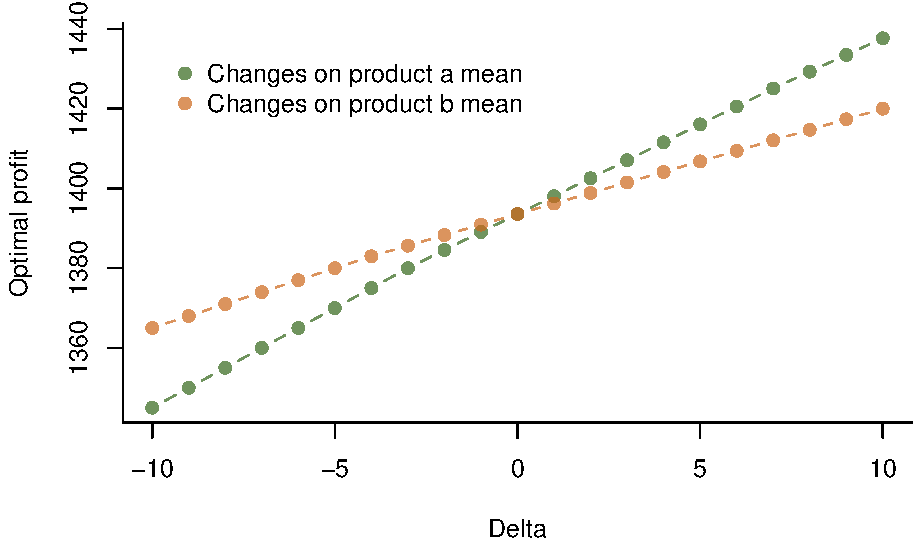
\includegraphics{Example-figure_files/figure-latex/mean-1.pdf}
\label{fig:mean}
\end{figure}

Surprisingly, one may find that increasing mean demand will actually increases optimal cost. That is because the ``cost" referred here is ``opportunity cost" \cite{Ch12,Po02}, which is incurred by \emph{not} gaining the benefit associated with the best alternative choice, e.g., the profit could have been earned. As one could notice in sensitivity reports, the time constraint on resource dimension $B$ is binding. Therefore, only promoting mean demand won't bring any gain to the retailer, but increases the demand-supply gap, and therefore, increases opportunity cost even more.

Instead, the retailer should concentrate on easing the binding constraint, in order to gain more supply power, and therefore meet the demand. Reversely, the retailer could also look into anti-promotion methods (if exist), that convert excess demand into cash flow, e.g., ``selling" customer to other retailers to get stable cash back.

One can compare these results with simulation outputs in Figure \ref{fig:mean} for verification.

On the other hand, we consider a decrease of standard deviation on estimated demand on product $a$ or $b$. Applying the formulation from Subsection \ref{sub:th-uncor}, we should have margin gain on decreasing standard deviation by $k\%$ as:
\[
\begin{aligned}
    \Delta \, P_a = -12.1 \, k_a,\\
    \Delta \, P_b = -22.1 \, k_b,
\end{aligned}
\]
providing the demand remain positive and variance is no less than zero. In this case, we can see that conducting market research may reduce cost. The simulated results are presented in Figure \ref{fig:var}. The retailer, therefore, could decide whether or not to use market research and to what extent should the research be used by comparing research cost and the margin gain.
\begin{figure}[htb]
\centering
\caption{Optimal cost vs. Change of variance}
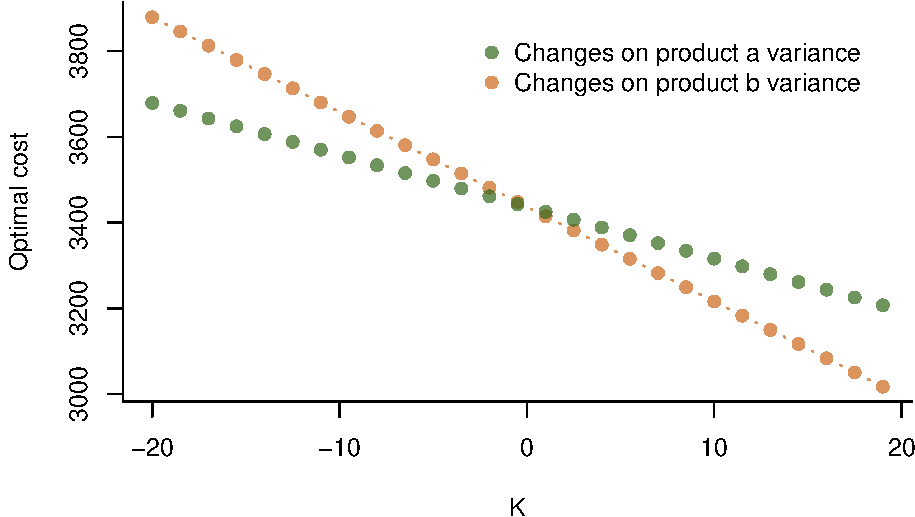
\includegraphics{Example-figure_files/figure-latex/var-1.pdf}
\label{fig:var}
\end{figure}

\subsection{Cross-price elasticities} \label{sub:app2}

We now suppose the demand of products are correlated, and the cross-price elasticity is known. According to traditional economics textbook \cite{Fr08}. The cross-price elasticity measures the responsiveness in the quantity demanded of one product when the price for another product changes. An elasticity $E_{ij} = -\omega$ means that each percent of selling price increase in product $j$ will causes $\omega$ percents of demand decrease in product $i$. Recall the demand formulation:
\[
\mathbf{\tilde{d}} =  \mathbf{\hat{M}} \mathbf{w}
+ \mathbf{\hat{N}} \mbox{\boldmath$\tilde{\epsilon}$}.
\]
We could allow the explanatory variable $\mathbf{w}$ to contain prices of all relevant products, and metrics $\mathbf{\hat{M}}$ to contain elasticities estimation. With the context of previous example, we let:
\[
\begin{aligned}
&\mathbf{\hat{M}} = 
\begin{pmatrix}
\alpha_a&\frac{E_{aa}}{p_a}\mu_a&\frac{E_{ab}}{p_b}\mu_a\\
\alpha_b&\frac{E_{ba}}{p_a}\mu_b&\frac{E_{bb}}{p_b}\mu_b
\end{pmatrix} =
\begin{pmatrix}
294&-15.75&7\\
189&10.5&-10.5
\end{pmatrix},\\
&\mathbf{w} = 
\begin{pmatrix}
1\\
p_a\\
p_b
\end{pmatrix} =
\begin{pmatrix}
1\\
8\\
6
\end{pmatrix}
\end{aligned}
\]
where set $E_{aa} = -0.6$, $E_{ab} = 0.2$, $E_{ba} = 0.4$ and $E_{bb} = -0.3$, while $\alpha_a$, $\alpha_b$ can be calculated by $\mbox{\boldmath$\mu$} = \mathbf{\hat{M}}\mathbf{w}$.

Moreover, we recall that the elements in \mbox{\boldmath$\tilde{\epsilon}$} are independent, and set
\[
\mathbf{\hat{N}} = 
\begin{pmatrix}
\hat{\sigma}_a^m&\hat{\sigma}_a&0\\
\hat{\sigma}_b^m&0&\hat{\sigma}_b\\
\end{pmatrix} =
\begin{pmatrix}
16.94&15.5&0\\
32.41&0&15.5\\
\end{pmatrix}
,\quad \mbox{\boldmath$\tilde{\epsilon}$} = 
\begin{pmatrix}
\tilde{\epsilon}_m\\
\tilde{\epsilon}_a\\
\tilde{\epsilon}_b
\end{pmatrix},
\]
where $\hat{\sigma}_a^m \tilde{\epsilon}_m$ and $\hat{\sigma}_b^m \tilde{\epsilon}_m$ represent the uncontrollable error of product $a$ and $b$, while $\hat{\sigma}_a \tilde{\epsilon}_a$ and $\hat{\sigma}_b \tilde{\epsilon}_b$
represent the reducible error due to inaccurate forecasts. We let $\hat{\sigma}_a = \hat{\sigma}_b$ in the setting since we assume there is no significant difference in the forecasting method used on each product.

We first consider the effect of marketing intervention on price setting. Suppose that by marketing intervention, the selling price of product $a$ or $b$ could be altered by $\Delta p_a$ and/or $\Delta p_b$. This change will now affect both the parameters of objective function and corresponding constraints (\ref{eq:over}) and (\ref{eq:under}). Recalling the margin can be computed by $\mbox{\boldmath$\delta$}^T \mathbf{x}^* + \mbox{\boldmath$\gamma$}^T \mbox{\boldmath$\pi$}^*$,
as long as the components of $\mbox{\boldmath$\delta$}$ and $\mbox{\boldmath$\gamma$}$
are ``sufficiently small”, we have: 


%%%%%%%%%%%%%%%%%%%%
\section{Summary}
\label{se:conclusion}
This paper provides a framework of applying LP sensitivity analysis on formulated MPNP. Specifically, we use SA technique to estimate the effect of changes in moments of demand distribution on the optimal cost. We first formulate the MPNP into a two-stage stochastic linear programming with recourse, which can be view as large LP model with finite scenarios. Then, we perform the non-standard SA to derive the margin. Therefore, as long as the changes in allowable range, we can inform the market decision directly.

In this paper, we considered two improvements that could alter the demand, each of which was then expressed mathematically. We can, therefore, decide whether to use those effort by comparing the gain and loss.

We also perform an example to demonstrate the approach. The result from our approach is in line with the simulation output.

%%%%%%%%%%%%%%%%%%%%%%%%%%%%%%
\printbibliography
%%%%%%%%%%%%%%%%%%%%%%%%%%%%%%
\newpage
\begin{center}
{\bf\Large Appendices}
\end{center}

\appendix

\section{Sensitivity Report: An Example}
\label{se:report}

\begingroup\fontsize{7}{9}\selectfont
\begin{longtable}{cccccc}
\caption{Sensitivity Report: Variable Cells}
\label{tab:sen_var}\\
\toprule
variable & final value & reduced cost & coefficient & allowable increase & allowable decrease\\
\midrule
\endfirsthead
\multicolumn{6}{@{}l}{\textit{(continued)}}\\
\toprule
variable & final value & reduced cost & coefficient & allowable increase & allowable decrease\\
\midrule
\endhead
\
\endfoot
\bottomrule
\endlastfoot
$y_a^{1}$ & 7.1 & 0.0 & -0.833 & 0.317 & 0.5\\
$y_a^{2}$ & 0.0 & -0.833 & -0.833 & 0.833 & 10000.0\\
$y_a^{3}$ & 27.1 & 0.0 & -0.833 & 0.317 & 0.5\\
$y_a^{4}$ & 17.1 & 0.0 & -0.833 & 0.317 & 0.5\\
$y_a^{5}$ & 17.1 & 0.0 & -0.833 & 0.317 & 0.5\\
\addlinespace
$y_a^{6}$ & 0.0 & -0.833 & -0.833 & 0.833 & 10000.0\\
$y_a^{7}$ & 0.0 & -0.833 & -0.833 & 0.833 & 10000.0\\
$y_a^{8}$ & 0.0 & -0.833 & -0.833 & 0.833 & 10000.0\\
$y_a^{9}$ & 7.1 & 0.0 & -0.833 & 0.317 & 0.5\\
$y_a^{10}$ & 17.1 & 0.0 & -0.833 & 0.317 & 0.5\\
\addlinespace
$y_a^{11}$ & 0.0 & -0.833 & -0.833 & 0.833 & 10000.0\\
$y_a^{12}$ & 0.0 & -0.833 & -0.833 & 0.833 & 10000.0\\
$y_b^{1}$ & 0.0 & -0.833 & -0.833 & 0.833 & 10000.0\\
$y_b^{2}$ & 0.0 & -0.833 & -0.833 & 0.833 & 10000.0\\
$y_b^{3}$ & 10.0 & 0.0 & -0.833 & 0.607 & 0.226\\
\addlinespace
$y_b^{4}$ & 30.0 & 0.0 & -0.833 & 0.607 & 0.226\\
$y_b^{5}$ & 0.0 & -0.607 & -0.833 & 0.607 & 10000.0\\
$y_b^{6}$ & 0.0 & -0.833 & -0.833 & 0.833 & 10000.0\\
$y_b^{7}$ & 40.0 & 0.0 & -0.833 & 0.607 & 0.226\\
$y_b^{8}$ & 60.0 & 0.0 & -0.833 & 0.607 & 0.226\\
\addlinespace
$y_b^{9}$ & 30.0 & 0.0 & -0.833 & 0.607 & 0.226\\
$y_b^{10}$ & 0.0 & -0.833 & -0.833 & 0.833 & 10000.0\\
$y_b^{11}$ & 0.0 & -0.833 & -0.833 & 0.833 & 10000.0\\
$y_b^{12}$ & 0.0 & -0.833 & -0.833 & 0.833 & 10000.0\\
$z_a^{1}$ & 0.0 & -0.083 & -0.083 & 0.083 & 10000.0\\
\addlinespace
$z_a^{2}$ & 12.9 & 0.0 & -0.083 & 0.083 & 0.317\\
$z_a^{3}$ & 0.0 & -0.083 & -0.083 & 0.083 & 10000.0\\
$z_a^{4}$ & 0.0 & -0.083 & -0.083 & 0.083 & 10000.0\\
$z_a^{5}$ & 0.0 & -0.083 & -0.083 & 0.083 & 10000.0\\
$z_a^{6}$ & 2.9 & 0.0 & -0.083 & 0.083 & 0.317\\
\addlinespace
$z_a^{7}$ & 32.9 & 0.0 & -0.083 & 0.083 & 0.317\\
$z_a^{8}$ & 42.9 & 0.0 & -0.083 & 0.083 & 0.317\\
$z_a^{9}$ & 0.0 & -0.083 & -0.083 & 0.083 & 10000.0\\
$z_a^{10}$ & 0.0 & -0.083 & -0.083 & 0.083 & 10000.0\\
$z_a^{11}$ & 2.9 & 0.0 & -0.083 & 0.083 & 0.317\\
\addlinespace
$z_a^{12}$ & 32.9 & 0.0 & -0.083 & 0.083 & 0.317\\
$z_b^{1}$ & 40.0 & 0.0 & -0.25 & 0.226 & 0.607\\
$z_b^{2}$ & 20.0 & 0.0 & -0.25 & 0.226 & 0.607\\
$z_b^{3}$ & 0.0 & -0.25 & -0.25 & 0.25 & 10000.0\\
$z_b^{4}$ & 0.0 & -0.25 & -0.25 & 0.25 & 10000.0\\
\addlinespace
$z_b^{5}$ & 0.0 & 0.0 & -0.25 & 0.226 & 0.607\\
$z_b^{6}$ & 0.0 & 0.0 & -0.25 & 0.226 & 0.607\\
$z_b^{7}$ & 0.0 & -0.25 & -0.25 & 0.25 & 10000.0\\
$z_b^{8}$ & 0.0 & -0.25 & -0.25 & 0.25 & 10000.0\\
$z_b^{9}$ & 0.0 & -0.25 & -0.25 & 0.25 & 10000.0\\
\addlinespace
$z_b^{10}$ & 10.0 & 0.0 & -0.25 & 0.226 & 0.607\\
$z_b^{11}$ & 50.0 & 0.0 & -0.25 & 0.226 & 0.607\\
$z_b^{12}$ & 50.0 & 0.0 & -0.25 & 0.226 & 0.607\\
$x_a$ & 207.1 & 0.0 & 5.0 & 0.317 & 0.5\\
$x_b$ & 210.0 & 0.0 & 3.0 & 0.607 & 0.226\\*
\end{longtable}
\endgroup{}

\begingroup\fontsize{6}{9}\selectfont
\begin{longtable}{cccccc}
\caption{Sensitivity Report: Constraints}
\label{tab:sen_con}\\
\toprule
row & final value & shadow price & constraint RHS & allowable increase & allowable decrease\\
\midrule
\endfirsthead
\multicolumn{6}{@{}l}{\textit{(continued)}}\\
\toprule
row & final value & shadow price & constraint RHS & allowable increase & allowable decrease\\
\midrule
\endhead
\
\endfoot
\bottomrule
\endlastfoot
time\_A & 2088.6 & 0.0 & 2200 & 10000.0 & 111.4\\
time\_B & 2500.0 & 0.071 & 2500 & 20.0 & 50.0\\
time\_C & 3337.1 & 0.0 & 3500 & 10000.0 & 162.9\\
over\_1\textasciicircum{}1 & 200.0 & 0.833 & 200 & 7.1 & 10000.0\\
over\_1\textasciicircum{}2 & 207.1 & 0.0 & 220 & 10000.0 & 12.9\\
\addlinespace
over\_1\textasciicircum{}3 & 180.0 & 0.833 & 180 & 27.1 & 10000.0\\
over\_1\textasciicircum{}4 & 190.0 & 0.833 & 190 & 17.1 & 10000.0\\
over\_1\textasciicircum{}5 & 190.0 & 0.833 & 190 & 17.1 & 10000.0\\
over\_1\textasciicircum{}6 & 207.1 & 0.0 & 210 & 10000.0 & 2.9\\
over\_1\textasciicircum{}7 & 207.1 & 0.0 & 240 & 10000.0 & 32.9\\
\addlinespace
over\_1\textasciicircum{}8 & 207.1 & 0.0 & 250 & 10000.0 & 42.9\\
over\_1\textasciicircum{}9 & 200.0 & 0.833 & 200 & 7.1 & 10000.0\\
over\_1\textasciicircum{}10 & 190.0 & 0.833 & 190 & 17.1 & 10000.0\\
over\_1\textasciicircum{}11 & 207.1 & 0.0 & 210 & 10000.0 & 2.9\\
over\_1\textasciicircum{}12 & 207.1 & 0.0 & 240 & 10000.0 & 32.9\\
\addlinespace
under\_1\textasciicircum{}1 & 207.1 & 0.0 & 200 & 7.1 & 10000.0\\
under\_1\textasciicircum{}2 & 220.0 & -0.083 & 220 & 10000.0 & 12.9\\
under\_1\textasciicircum{}3 & 207.1 & 0.0 & 180 & 27.1 & 10000.0\\
under\_1\textasciicircum{}4 & 207.1 & 0.0 & 190 & 17.1 & 10000.0\\
under\_1\textasciicircum{}5 & 207.1 & 0.0 & 190 & 17.1 & 10000.0\\
\addlinespace
under\_1\textasciicircum{}6 & 210.0 & -0.083 & 210 & 10000.0 & 2.9\\
under\_1\textasciicircum{}7 & 240.0 & -0.083 & 240 & 10000.0 & 32.9\\
under\_1\textasciicircum{}8 & 250.0 & -0.083 & 250 & 10000.0 & 42.9\\
under\_1\textasciicircum{}9 & 207.1 & 0.0 & 200 & 7.1 & 10000.0\\
under\_1\textasciicircum{}10 & 207.1 & 0.0 & 190 & 17.1 & 10000.0\\
\addlinespace
under\_1\textasciicircum{}11 & 210.0 & -0.083 & 210 & 10000.0 & 2.9\\
under\_1\textasciicircum{}12 & 240.0 & -0.083 & 240 & 10000.0 & 32.9\\
over\_2\textasciicircum{}1 & 210.0 & 0.0 & 250 & 10000.0 & 40.0\\
over\_2\textasciicircum{}2 & 210.0 & 0.0 & 230 & 10000.0 & 20.0\\
over\_2\textasciicircum{}3 & 200.0 & 0.833 & 200 & 10.0 & 10000.0\\
\addlinespace
over\_2\textasciicircum{}4 & 180.0 & 0.833 & 180 & 30.0 & 10000.0\\
over\_2\textasciicircum{}5 & 210.0 & 0.226 & 210 & 0.0 & 4.0\\
over\_2\textasciicircum{}6 & 210.0 & 0.0 & 210 & 10000.0 & 0.0\\
over\_2\textasciicircum{}7 & 170.0 & 0.833 & 170 & 40.0 & 10000.0\\
over\_2\textasciicircum{}8 & 150.0 & 0.833 & 150 & 60.0 & 10000.0\\
\addlinespace
over\_2\textasciicircum{}9 & 180.0 & 0.833 & 180 & 30.0 & 10000.0\\
over\_2\textasciicircum{}10 & 210.0 & 0.0 & 220 & 10000.0 & 10.0\\
over\_2\textasciicircum{}11 & 210.0 & 0.0 & 260 & 10000.0 & 50.0\\
over\_2\textasciicircum{}12 & 210.0 & 0.0 & 260 & 10000.0 & 50.0\\
under\_2\textasciicircum{}1 & 250.0 & -0.25 & 250 & 10000.0 & 40.0\\
\addlinespace
under\_2\textasciicircum{}2 & 230.0 & -0.25 & 230 & 10000.0 & 20.0\\
under\_2\textasciicircum{}3 & 210.0 & 0.0 & 200 & 10.0 & 10000.0\\
under\_2\textasciicircum{}4 & 210.0 & 0.0 & 180 & 30.0 & 10000.0\\
under\_2\textasciicircum{}5 & 210.0 & -0.25 & 210 & 10000.0 & 0.0\\
under\_2\textasciicircum{}6 & 210.0 & -0.25 & 210 & 10000.0 & 0.0\\
\addlinespace
under\_2\textasciicircum{}7 & 210.0 & 0.0 & 170 & 40.0 & 10000.0\\
under\_2\textasciicircum{}8 & 210.0 & 0.0 & 150 & 60.0 & 10000.0\\
under\_2\textasciicircum{}9 & 210.0 & 0.0 & 180 & 30.0 & 10000.0\\
under\_2\textasciicircum{}10 & 220.0 & -0.25 & 220 & 10000.0 & 10.0\\
under\_2\textasciicircum{}11 & 260.0 & -0.25 & 260 & 10000.0 & 50.0\\
\addlinespace
under\_2\textasciicircum{}12 & 260.0 & -0.25 & 260 & 10000.0 & 50.0\\*
\end{longtable}
\endgroup{}


\end{document}